\documentclass[10pt, a4paper, hidelinks]{article}
\usepackage[paper=a4paper, left=2cm, right=2cm, bottom=2cm, top=3cm]{geometry} %ajustar márgnens
\usepackage[utf8]{inputenc}
\usepackage[spanish]{babel}
\usepackage{caratula}
\usepackage{enumitem} 
\usepackage{hyperref}
\usepackage{mathtools}
\usepackage[font=small,labelfont=bf]{caption}
\newcommand\floor[1]{\lfloor#1\rfloor}
\newcommand\ceil[1]{\lceil#1\rceil}
%\usepackage{clrscode3e} Estilo Cormen
\usepackage[spanish,onelanguage,ruled,vlined,nofillcomment]{algorithm2e}
\usepackage{algpseudocode}
\usepackage{xcolor}
\usepackage[final]{pdfpages} % para agregar el enunciado
%%%%%%%%%%%%%% Formato de párrafos %%%%%%%%%%%%%%%%%%
\setlength{\parindent}{2em}
\setlength{\parskip}{3pt}
%%%%%%%%%%%%%%%%%%%%%%%%%%%%%%%%%%%%%%%%%%%%%%%%%%%%%%%
\usepackage{fancyhdr}
\usepackage{lastpage}
\setlength{\intextsep}{0.2cm}
\pagestyle{fancy}
\lhead{Sistemas Operativos}
\rhead{$1^{\mathrm{er}}$ cuatrimestre de 2018}

\LinesNumbered
\DontPrintSemicolon

\newcommand{\comp}[1]{$\mathcal{O}(#1)$}

%%%%%%%%%%%%%%%%%%% Macro para comentar codigo %%%%%%%%%%%%%%%%%%%%%%%%%
\newcommand{\comentario}[1]{
\SetKwComment{Comment}{/* }{ */}
\textcolor{blue}{\Comment*[h]{{#1}}}
}
%%%%%%%%%%%%%%%%%%%%%%%%%%%%%%%%%%%%%%%%%%%%%%%%%%%%%%%%%%%%%%%%%%%%%%%%

\begin{document}

\materia{Sistemas Operativos}
\submateria{Primer cuatrimestre del 2018}
\titulo{Trabajo Práctico 2: \texttt{blockchain}}
\integrante{Budiño, Gabriel Fabricio}{046/16}{gabriel.f.budi@gmail.com} % obligatorio 
\integrante{Garro, Damián Eugenio}{354/16}{damian.garro.mst@gmail.com} % obligatorio 
\integrante{Rozenberg, Uriel Jonathan}{838/12}{rozenberguriel@gmail.com} % obligatorio 

\maketitle

\tableofcontents
\pagenumbering{gobble}

\pagebreak
\pagenumbering{arabic}
\cfoot{\thepage /\pageref{LastPage}}

\section{Introducción}
Para este trabajo se debía implementar una cadena de bloques ($blockchain$) utilizando la interfaz MPI con el objetivo de desarrollar conocimientos en sistemas distribuidos.

A continuación se presenta un breve resumen de la resolución de cada ejercicio así como de la experimentación realizada. El enunciado completo se encuentra en el Apéndice A, donde puede consultarse tanto la información de las estructuras usadas como los enunciados a los que responden las siguientes secciones del informe.

\section{Resolución}
\subsection{Ejercicio 1}
La función \texttt{broadcast\_block} es la encargada de, al momento en que un nodo mina exitosamente un bloque, comunicárselo al resto. El pseudocódigo de la misma es el siguiente:

\begin{algorithm}[H]
\SetKwProg{Fn}{Función}{}{fin}
\SetAlgoLined
\Fn{broadcast\_block(bloque)}{
	\ForEach{nodo n distinto del productor del bloque}{
		\texttt{MPI\_Send}($bloque$, $n.rank$, \texttt{TAG\_NEW\_BLOCK}) \\
	}
}
\caption{\texttt{broadcast\_block}}
\end{algorithm}

Para referenciar a un proceso ($nodo$) usamos su \texttt{rank} dentro del communicator global \texttt{MPI\_COMM\_WORLD}. Cada nodo metiene las variables \texttt{mpi\_rank} y \texttt{total\_nodes}. Así, para cada 1 $\leq i \leq$ \texttt{total\_nodes}, definimos $destino$ como $(i + \texttt{mpi\_rank})$ $mod$ \texttt{total\_nodes} y enviamos el mensaje usando \texttt{MPI\_Send} con $destino$, $bloque$ y el tag \texttt{TAG\_NEW\_BLOCK} como parámetros (principalmente). Es decir, enviamos el bloque desde el nodo siguiente al que lo minó en adelante, asegurándonos así que todos los nodos envíen mensajes en distinto orden.
 
\subsection{Ejercicio 2}
Para la resolución de este ejercicio, se agregó a la información que mantiene cada nodo un bool atómico \texttt{probando}, con el cual se implementó un $spinlock$. Se pedía modificar las funciones \texttt{node} y \texttt{proof\_of\_work} para evitar $race$ $conditinos$. A continuación, se muestra el pseudocódigo de la parte implementada del método \texttt{node}:

\begin{algorithm}[H]
\SetKwProg{Fn}{Función}{}{fin}
\SetAlgoLined
\Fn{node()}{
	\comentario{Tomar valor de mpi\_rank y de total\_nodes} \\
	\comentario{Inicialización del primer bloque} \\
	\comentario{Crear thread para minar} \\
	crear nuevo thread con la función \texttt{proof\_of\_work} como punto de inicio \\
	\While{\texttt{true}}{
		\comentario{Recibir mensajes de otros nodos} \\
		$status$ $\leftarrow$ \texttt{MPI\_Probe()} \\
		\comentario{Si es un mensaje de nuevo bloque} \\
		\If{status.tag = \texttt{TAG\_NEW\_BLOCK}}{
			$status$ $\leftarrow$ \texttt{MPI\_Recv($block$)} \\
			\texttt{lock()} \\
			\texttt{validate\_block\_for\_chain}($block$, $status$) \\
			\texttt{unlock()}
		} \comentario{Si es un mensaje de pedido de cadena} \\
		\ElseIf{status.tag = TAG\_CHAIN\_HASH}{
			$status$ $\leftarrow$ \texttt{MPI\_Recv($block\_hash$)} \\
			\texttt{mandar\_cadena}($block\_hash$, $status$) \\
		}
	}
}
\caption{\texttt{node}}
\end{algorithm}

Ya que el mensaje recibido puede contener un bloque minado por otro o un hash para solicitar una cadena, y estos tienen tipos diferentes, antes de llamar a la función \texttt{MPI\_Recv} se llama a \texttt{MPI\_Probe()} para verificar el $tag$ del próximo mensaje recibido y a partir de éste usar \texttt{MPI\_Recv} con el tipo de dato correcto.

Si se recibe un mensaje con $tag$ \texttt{TAG\_CHAIN\_HASH} entonces se invoca a la función \texttt{mandar\_cadena} que manda la cadena al nodo que la solicitó. Para eso, la misma crea un arreglo de bloque cuyo tamaño (en cantidad) es el mínimo entre \texttt{VALIDATION\_BLOCKS} y el índice del bloque del hash solicitada. A continuación llena el arreglo, en la primera posición con el bloque del hash recibido y en las siguientes con los bloques anteriores. Los bloques los obtiene usando el diccionario \texttt{node\_blocks}.

En cuanto a la función \texttt{proof\_of\_work}, una vez que se consigue la cantidad de ceros requerida por la dificultad configurada, se ejecuta un bloque que inicialmente verifica que no haya cambiado \texttt{last\_block\_in\_chain} y finalmente llama a \texttt{broadcast\_block} para comunicar que se ha minado un bloque. Consideramos estas dos acciones como los límites de la sección crítica, así que llamamos a \texttt{lock()} inmediatamente antes de la primera y a \texttt{unlock()} inmediatamente después de la segunda, de esta forma evitamos \textit{race conditions} porque la cadena del nodo solo puede ser modificada por un \textit{thread} al mismo tiempo

\subsection{Ejercicio 3}
Cuando un nodo mine un nuevo bloque y le avise al resto, estos deberán decidir si agregarlo o no a la cadena. Para eso se utiliza la función \texttt{validate\_block\_for\_chain}, la cual debía cumplir con el consenso definido en la sección 3 del enunciado. Su pseudocódigo es el siguiente:

\begin{algorithm}[H]
\SetKwProg{Fn}{Función}{}{fin}
\SetAlgoLined
\Fn{validate\_block\_for\_chain(rBlock, status)}{
	\If{\texttt{valid\_new\_block(rBlock)}}{
		agrego $rBlock$ a \texttt{node\_blocks} \\
		\If{rBlock.indice = 1 y \texttt{last\_block\_in\_chain}.indice = 0}{
			\comentario{2do item del consenso} \\
			\texttt{last\_block\_in\_chain} $\leftarrow$ $rBlock$ \\
			devolver \texttt{true}
		}
		\If{rBlock.indice = \texttt{last\_block\_in\_chain}.indice + 1}{
			\uIf{anterior de rBlock = anterior de \texttt{last\_block\_in\_chain}}{
				\comentario{3er item del consenso} \\
				\texttt{last\_block\_in\_chain} $\leftarrow$ $rBlock$ \\
				devolver \texttt{true} \\			
			} \Else {
				\comentario{4to item del consenso} \\ 
				devolver \texttt{verificar\_y\_migrar\_cadena}($rBlock$, $status$)
			}
		}
		\If{rBlock.indice = \texttt{last\_block\_in\_chain}.indice}{
			\comentario{5to item del consenso} \\
			devolver \texttt{false}		
		}
		\If{rBlock.indice $<$ \texttt{last\_block\_in\_chain}.indice}{
			devolver \texttt{false}		
		}
		\If{rBlock.indice $>$ \texttt{last\_block\_in\_chain}.indice}{
			\comentario{6to item del consenso} \\
			devolver \texttt{verificar\_y\_migrar\_cadena}($rBlock$, $status$) \\
		}
	}
	\comentario{1er item del consenso} \\
	devolver \texttt{false}
}
\caption{\texttt{validate\_block\_for\_chain}}
\end{algorithm}

Esta función puede modificar \texttt{last\_block\_in\_chain} a salvo de \textit{race conditions} porque se llama dentro de la sección crítica que definimos en el ejercicio anterior. 
 
\subsection{Ejercicio 4}
Llegado al caso donde un nodo deba migrar a la $blockchain$ de otro, se utilizará la función \texttt{verificar\_y\_migrar\_cadena}. La misma debía cumplir con el protocolo descripto en la sección 4 del enunciado. A continuación se muestra su pseudocódigo:

\begin{algorithm}[H]
\SetKwProg{Fn}{Función}{}{fin}
\SetAlgoLined
\Fn{\texttt{verificar\_y\_migrar\_cadena}(rBlock, status)}{
	\comentario{Solicitud de los bloques} \\	
	\texttt{MPI\_Send}($rBlock.hash$, $status.mpi\_source$, \texttt{TAG\_CHAIN\_HASH}) \\
	\comentario{Recepción de los bloques} \\
	$blockchain$ $\leftarrow$ nuevo arreglo de bloques \\
	\texttt{MPI\_Recv}($blockchain$, $status.mpi\_source$, \texttt{TAG\_CHAIN\_RESPONSE}) \\
	\comentario{1er item del protocolo} \\
	\If{el primer elemento de $blockchain$ tiene índice o hash distinto al pedido}{
		devolver \texttt{false}	
	}
	\ForEach{bloque b $\in$ blockchain}{
		\comentario{2do item del protocolo} \\
		\If{el hash de b es válido}{
			devolver \texttt{false}	
		}
		$b'$ $\leftarrow$ siguiente del bloque b en blockchain \\
		\comentario{3er item del protocolo} \\		
		\If{hash del anterior de b $\neq$ b'.hash}{
			devolver \texttt{false}			
		}
		\comentario{4to item del protocolo} \\
		\If{b.indice $\neq$ b'.indice + 1}{
			devolver \texttt{false}		
		}	
	}
	$u$ $\leftarrow$ ultimo bloque de $blockchain$ \\
	\If{ningún b $\in$ blockchain está en el diccionario $\land$ $u$.indice $\neq$ 1}{
		devolver \texttt{false}		
	}
	agregar bloques recibidos a \texttt{node\_blocks} \\
	\texttt{last\_block\_in\_chain} $\leftarrow$ primer bloque de $blockchain$ \\
	devolver \texttt{true}	
}
\caption{\texttt{verificar\_y\_migrar\_cadena}}
\end{algorithm}

El arreglo $blockchain$ se crea con tamaño \texttt{VALIDATION\_BLOCKS} y en \texttt{MPI\_Recv} se especifica este valor para la cantidad máxima de bloques recibidos. Sin embargo, se pueden recibir menos y por eso utilizamos la función \texttt{MPI\_Get\_count} para saber la cantidad de bloques recibida. 

En cuanto al segundo ítem de verificaciones del conceso, el enunciando especifica que ``El hash del bloque recibido es igual al calculado por la función \texttt{block\_to\_hash}.''. Lo que hicimos en cambio fue revisar que el hash además resuelva el problema usando la función \texttt{solves\_problem}, y la verificación la hacemos para todos los bloques recibidos, no solo uno.

Esta función se llama solo desde la \texttt{validate\_block\_for\_chain}, la cual ya dijimos que se ejecuta dentro de la sección crítica, así que no hay \textit{race conditions} con el \textit{thread} que mina bloques.

\subsection{Ejercicio 5}

En el protocolo implementado es posible que se produzca una bifurcación de blockchains que nunca converjan. Supongamos el caso en que dos nodos, $alice$ y $bob$, minan bloques propios antes de recibir el mensaje correspondiente del otro. Ante esto, los bloques se crearán con igual índice y ambos nodos no tomarán acciones al recibir el mensaje del otro (pseudocódigo de \texttt{validate\_block\_for\_chain}, $5^{to}$ item del consenso), repitiendo por ejemplo la siguiente secuencia:

\begin{itemize}
	\itemsep0em
    \item $alice$ mina bloque de índice $i$ y lo agrega a su cadena.
    \item $bob$ mina bloque de índice $i$ y lo agrega a su cadena.
	\item $bob$ recibe bloque de índice $i$ de $alice$ y lo descarta.
	\item $alice$ recibe bloque de índice $i$ de $bob$ y lo descarta.    
\end{itemize}
 
Si dicha situación persiste hasta que sus blockchains superen en logitud a la constante \texttt{VALIDATION\_BLOCKS}, sus cadenas ya no podrán converger pues no se pueden migrar cadenas que superen esa longitud.
    
La demora o la pérdida de paquetes facilita que se de la situación antes mencionada. Los nodos, al enterarse tarde o directamente no enterarse de las acciones del resto, pueden caer en conflictos de consenso y así las blockchains de dos o más nodos pueden ir difiriendo hasta que ya no sea posible la convergencia. Particularmente, la demora de paquetes puede tener dos efectos distintos, o bien le puede dar suficiente tiempo a un nodo para que mine un bloque de un índice igual a uno que pudo haber recibido antes de otro nodo, o bien puede hacer que los bloques cuando sean recibidos sean tan viejos que se consideren inválidos por \texttt{valid\_new\_block} y se descarten. Cabe resaltar que el protocolo implementado no tiene como característica priorizar la convergencia, pues el envío de los bloques se hace sin una verificación de su recepción, cuando podría ser un caso a tener en cuenta para poder tomar acciones.  

También se observa que a mayor dificultad resulta más difícil minar exitosamente un bloque, bajo esta condición es más probable que cuando un nodo mine un bloque el resto lo reciba y lo agregue a sus cadenas antes de que otro mine uno distinto, por lo que sería esperable que todos los nodos tengan la misma cadena, facilitando así la convergencia. Por otro lado, a menor dificultad, los bloques se minarían con mayor frecuencia, así que de este modo sería probable que se produzcan más migraciones y más conflictos suaves, atentando así contra la convergencia del mismo modo ya discutido en esta sección.

Además, mientras más nodos tenga la red, los bloques se minarían con mayor frecuencia. En este protocolo la cantidad de nodos es establecida desde el inicio, pero en uno en donde se permita que más nodos ingresen a la red se tendría otro factor que varíe la cantidad de bloques minados por unidad de tiempo. En un sistema así, para mantener una frecuencia de minado constante se puede variar la $dificultad$ como lo hace $Bitcoin$, donde se modifica cada 2016 bloques según el tiempo que llevó minarlos. Siendo el objetivo 10 minutos por bloque (es decir, 20160 minutos para 2016 bloques), la dificultad se aumenta o reduce según la siguiente fórmula(llamando $tiempo$ a la cantidad de minutos que tomó minar los últimos 2016 bloques):

\begin{equation*}
dificultad\_nueva = dificultad\_vieja \times \frac{20160}{tiempo}
\end{equation*}

Esto no solo contempla el hecho de que la cantidad de nodos en la red varíe, sino también a que cada vez las computadoras tienen mayor poder de cómputo, por lo que también por esto es necesario ajustar la dificultad e históricamente la misma suele subir.\footnote{\url{https://bitinfocharts.com/comparison/bitcoin-difficulty.html}}
 
Con el fin de tener evidencia empírica de que los conflictos aumentan a menor dificultad o mayor cantidad de nodos, llevamos a cabo un experimento. En el mismo hicimos ejecuciones con distintos valores de dificultad (5, 10 y 15) y cantidad de nodos (5, 10, 20 y 50), haciendo 10 repeticiones por cada combinación y contando la cantidad de conflictos suaves en cada una (es decir, cuántas veces un nodo rechanza bloques por tener índice menor o igual a su último).

Para que las ejecuciones terminen hicimos que cuando un nodo mine un bloque de índice \texttt{MAX\_BLOCKS} (200 en nuestro caso), use la función \texttt{MPI\_Abort}, y de esta forma tener un log de eventos hasta este punto para poder analizar. 

Además, consideramos que también las ejecuciones pueden interrumpirse por algún error en funciones de MPI, sobre todo en los casos más exhaustivos (muchos nodos y poca dificultad), por lo que estos logs los ignoramos y repetimos la ejecución hasta tener una exitosa.

\begin{center}.
   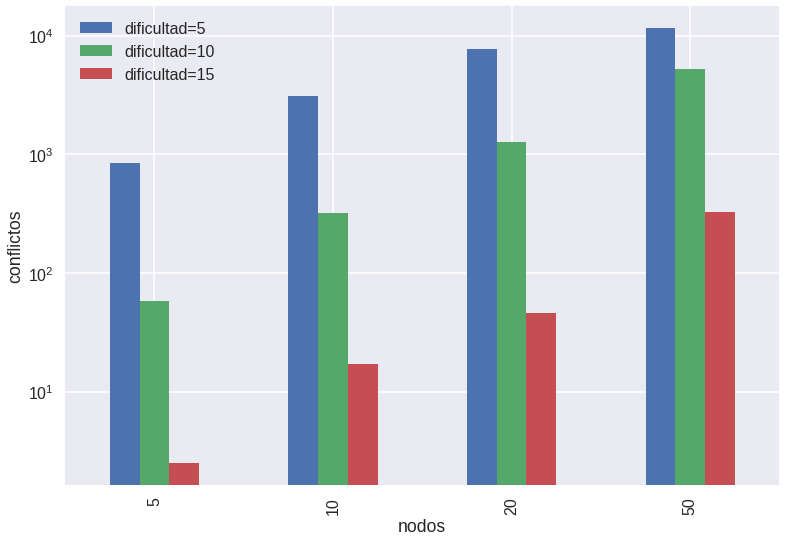
\includegraphics[height=9cm]{img/exp.png}
   \captionof{figure}{Cantidad promedio de conflictos suaves para distintas dificultades y cantidad de nodos.}
   \label{fig:exp}
\end{center}

A partir de la \textbf{Figura \ref{fig:exp}}, vemos que nuestras hipótesis parecen ser ciertas, el eje vertical muestra en escala logarítmica la cantidad en promedio de conflictos suaves de las ejecuciones según la dificultad y cantidad de nodos.




\newpage
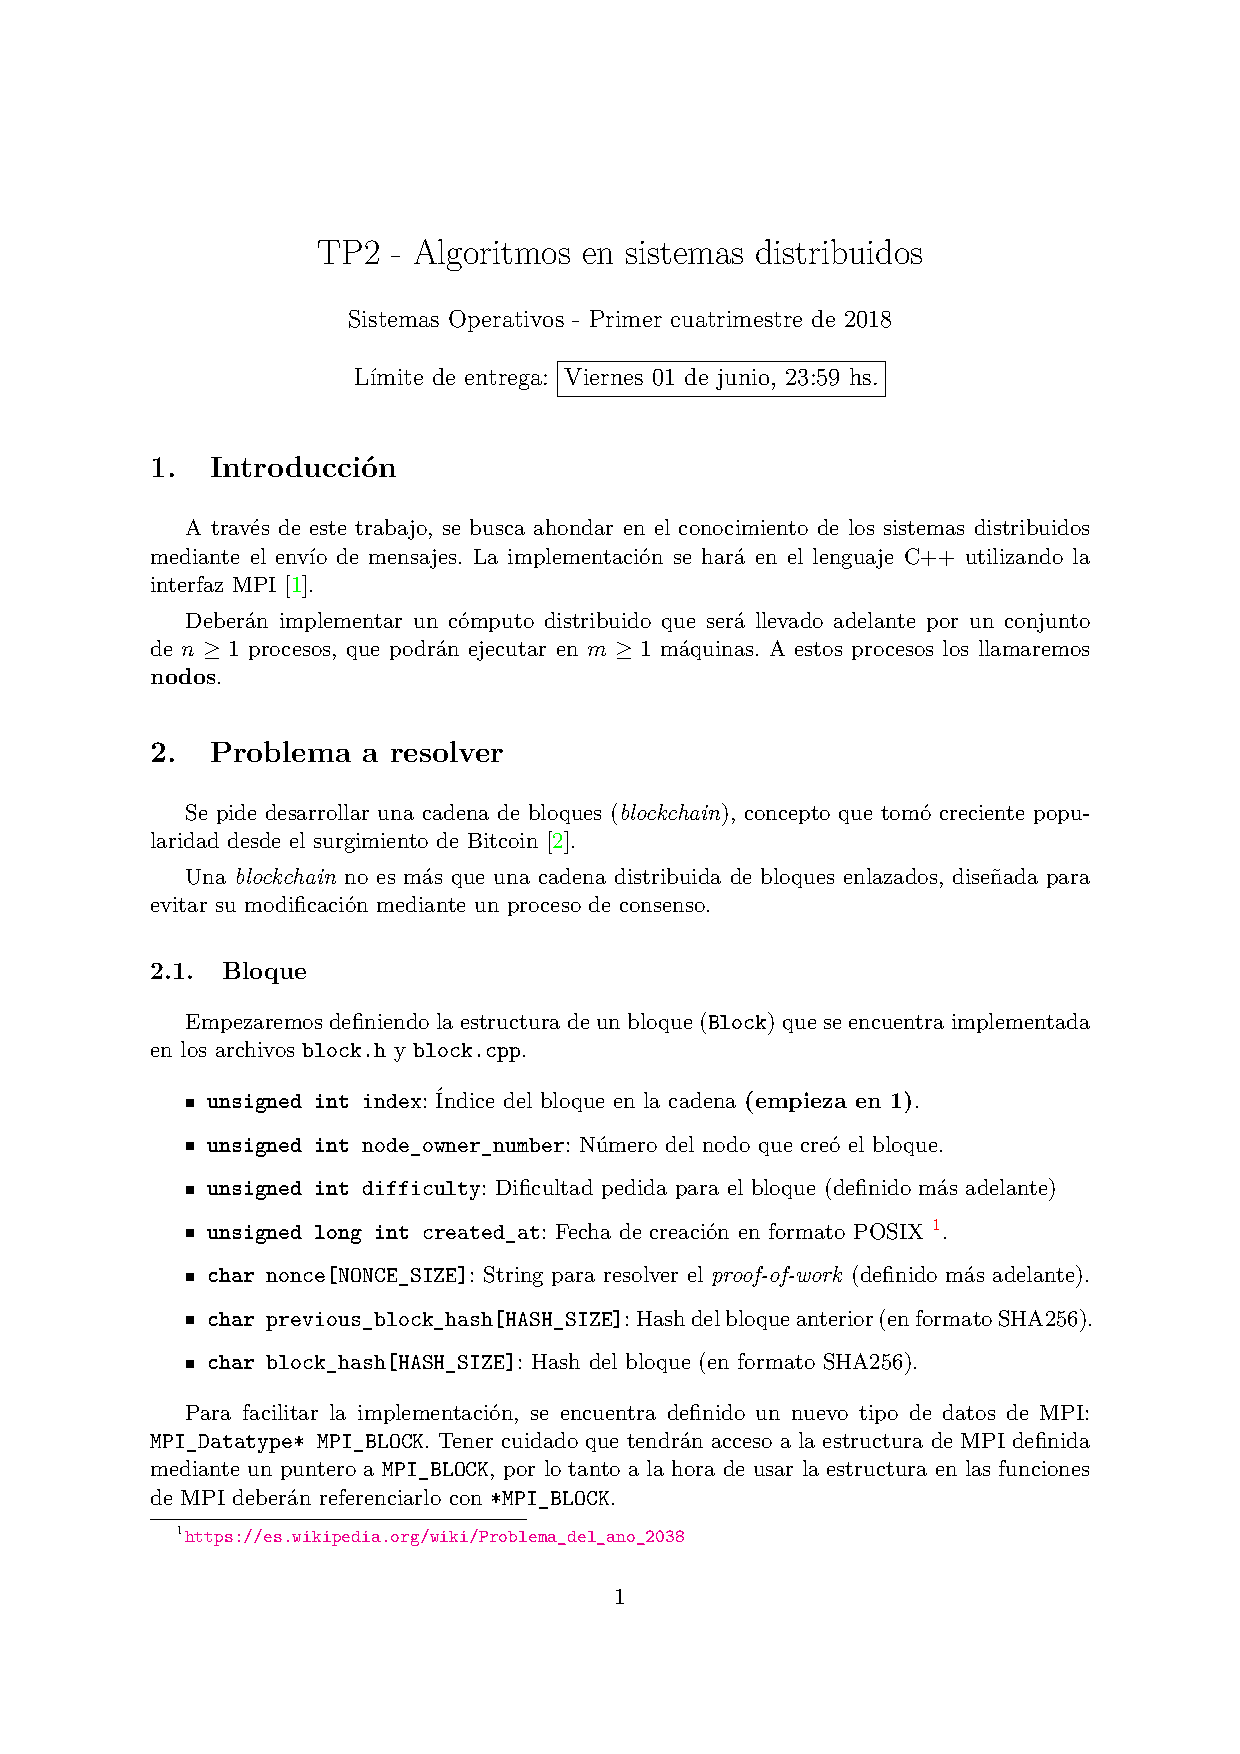
\includepdf[scale=0.75,pages=1,pagecommand=\section{Apéndices}
\subsection{Apéndice A - Enunciado}]{../enunciado.pdf}
\includepdf[scale=0.75,pages=2-,pagecommand=]{../enunciado.pdf}

\end{document}

